\documentclass[12pt,a4paper]{article}
\usepackage{import}
\usepackage{amsmath}
\usepackage{amsfonts}
\usepackage{amssymb}
\usepackage[toc,page]{appendix}
\usepackage{float}
%\usepackage{cmbright} %Computer modern bright font
\usepackage[T1]{fontenc}
%\usepackage{tgtermes}
\usepackage{newtxtext}
\usepackage{newtxmath}
%\usepackage[bitstream-charter]{mathdesign} %Bitstream charter font
%\usepackage[adobe-utopia]{mathdesign} %adobe utopia font
\usepackage{graphicx}
\usepackage{titlesec}
%\usepackage{braket}
\usepackage{physics}
\usepackage{pdfpages}

\newtheorem{mydef}{Def.}

\newcommand{\eq}[2]{\begin{equation} #2 \label{#1} \end{equation}}
\newcommand{\eqd}[2]{\begin{dmath} #2 \label{#1} \end{dmath}}
\newcommand{\eqa}[2]{\begin{equation}\begin{aligned} #2 \label{#1} \end{aligned}\end{equation}}

\renewcommand{\v}[1]{\mathbf{#1}}

\newcommand{\bm}[1]{\mathbf{#1}}

\renewcommand{\i}{\text{i}}
%\newcommand{\ssection}[1]{%
%  \section[#1]{\centering\normalfont\scshape #1}}
%\newcommand{\ssubsection}[1]{%
%  \subsection[#1]{\raggedright\normalfont\itshape #1}}

\newcommand{\vx}{\v{x}}
\newcommand{\ve}{\v{e}}
\newcommand{\vw}{\v{w}}

\newcommand{\levciv}{\epsilon_{ijk}}
%Set equation numbering 
\numberwithin{equation}{section}

\begin{document}

\author{Anton Ljungdahl, \\
\small{anton.ljungdahl@fysik.su.se}}
\title{Notes on angular momentum in quantum mechanics}
\date{\today}
\maketitle
\tableofcontents
\section{Commutation relations}
\import{./}{angmom1_v2.tex}

\appendix++
\section{Pen-and-paper calculations}
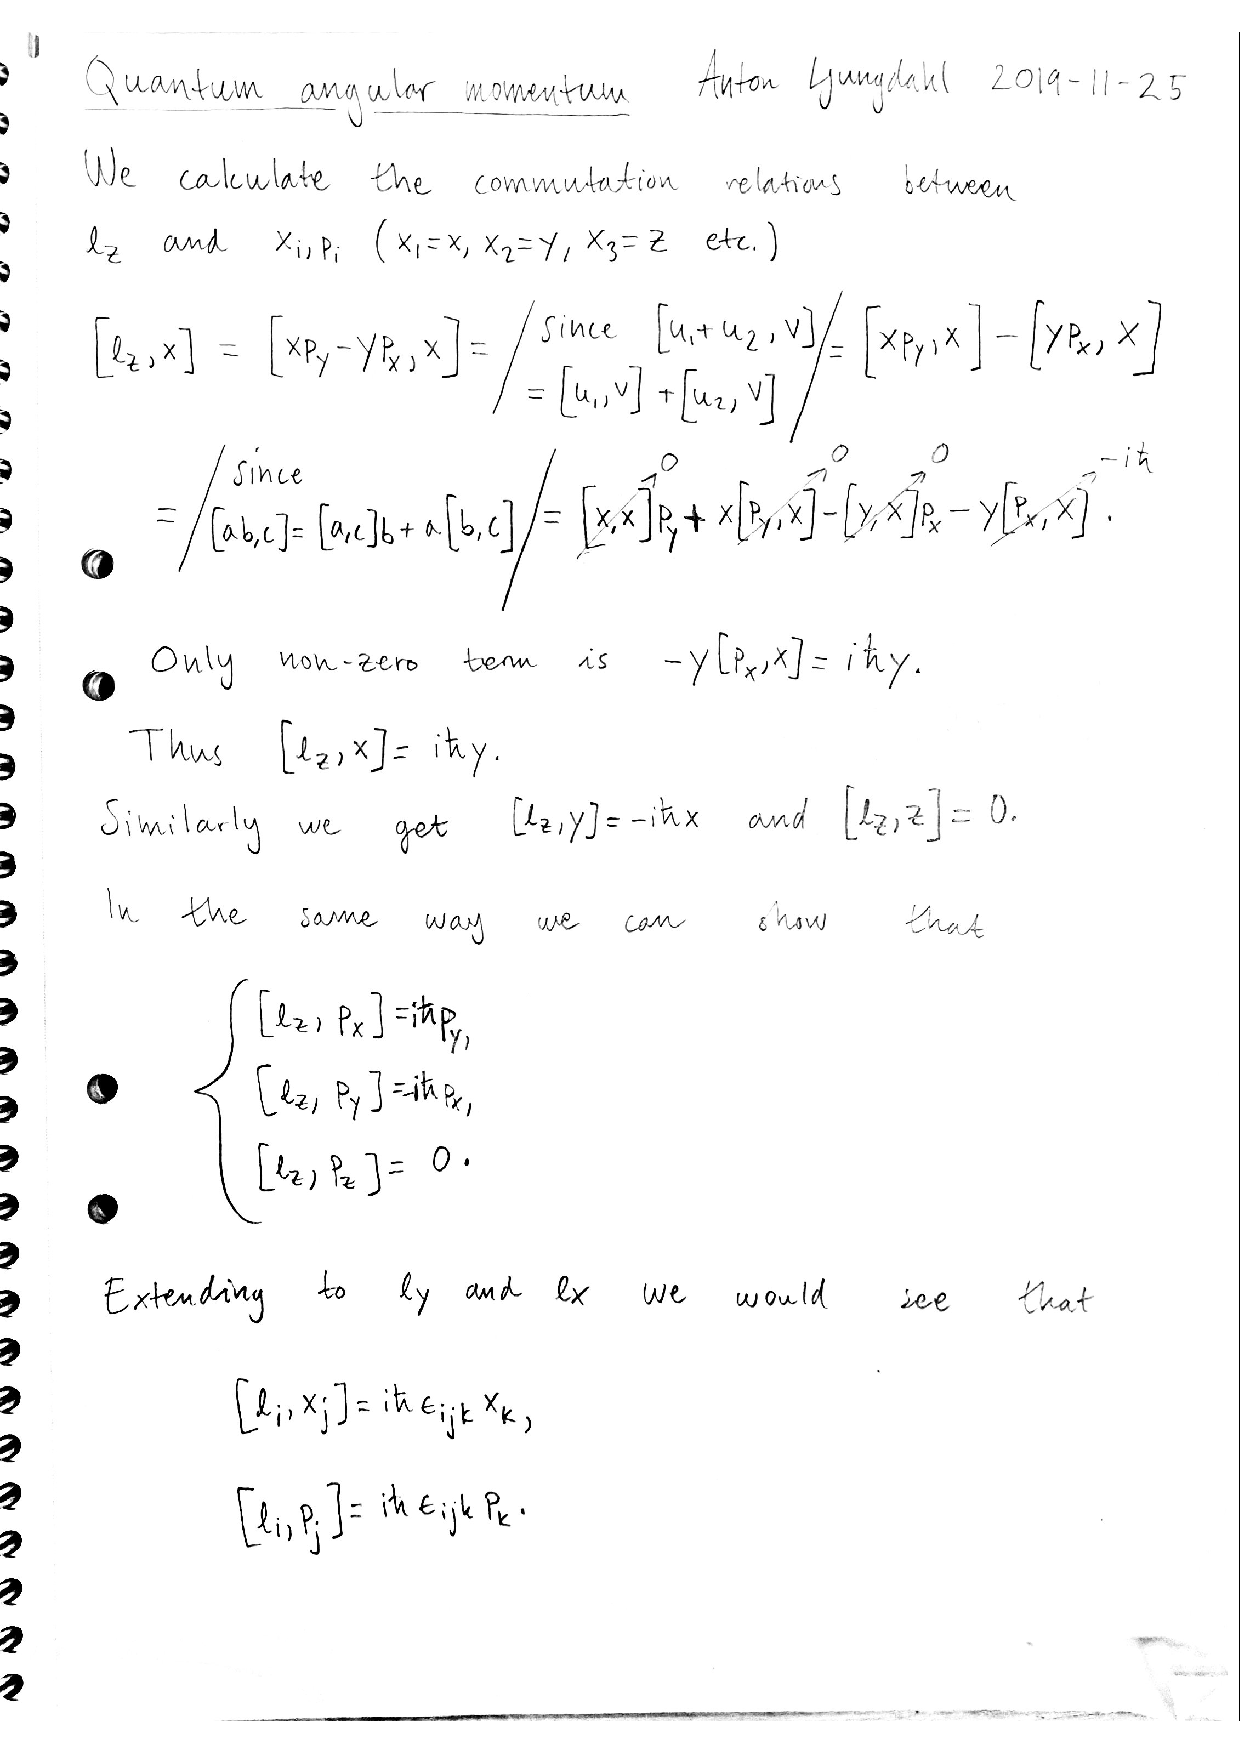
\includepdf[pages=-]{byhand_commutation_relations1.pdf}
\end{document}

%--------------------------------------------------------------------
